\documentclass[letterpaper,10pt,titlepage,journal,compsoc,draftclsnofoot,onecolumn]{IEEEtran}
\linespread{1}
\newcommand\tab[1][1cm]{\hspace*{#1}}
\usepackage{graphicx}                                        
\usepackage{amssymb}                                         
\usepackage{amsmath}                                         
\usepackage{amsthm}                                          

\usepackage{alltt}                                           
\usepackage{float}
\usepackage{color}
\usepackage{url}
\usepackage{listings}

\usepackage{balance}
\usepackage[TABBOTCAP, tight]{subfigure}
\usepackage{enumitem}
\usepackage{pstricks, pst-node}

\usepackage{geometry}
\usepackage{titling}
\geometry{textheight=8.5in, textwidth=6in}


\newcommand{\cred}[1]{{\color{red}#1}}
\newcommand{\cblue}[1]{{\color{blue}#1}}

\usepackage{hyperref}
\usepackage{geometry}

\def\name{James O'Neal}


%% The following metadata will show up in the PDF properties
\hypersetup{
  colorlinks = true,
  urlcolor = black,
  pdfauthor = {\name},
  pdfkeywords = {cs462 ''Senior Capstone''},
  pdftitle = {CS 462 Senior Capstone: Winter Progress},
  pdfsubject = {CS462 Senior Capstone},
  pdfpagemode = UseNone
}

\title{Energy Effeciency Center Website: \\ Winter Progress Report}
\author{James O'Neal}

\begin{document}
\begin{titlingpage}
    \maketitle
	\centering{}
    \begin{abstract}
        
        OSU’s Energy Efficiency Center help manufacturing and industrial companies increase their productivity and reduce their energy footprint by producing reports for energy and productivity recommendations. These reports, projects and funds are maintained in their website. The website has been developed and maintained by several programmers. As a result, the website has become disorganized, difficult to update and use. In order to remedy these issues we will design a secure, user friendly website with good code practices for the Energy Efficiency Center. 	Furthermore, the website is not accessible from mobile devices which decreases productivity while on the job site. With enough time, we would like to create a secure mobile app for the client which they are able to remotely access.
        
    \end{abstract}
\end{titlingpage}

\newpage

\tableofcontents{}

\newpage


\section{Purpose and Goals}

\tab OSU’s Energy Efficiency Center helps manufacturing and industrial companies reduce their energy footprint. This is accomplished by producing reports about energy trends and making recommendations based on them. The reports, projects, and other data are maintained in their internal website. The website has been developed by different programmers and as a result has become disorganized and difficult to update. In order to remedy these issues we will design a secure, user friendly website with good code practices for the Energy Efficiency Center. Furthermore, the website is not accessible from mobile devices which decreases productivity of workers who can’t access the website while on the job site. We aim to create a website that is mobile accessible and friendly for increased accessibility.

\section{Current Progress}

\tab
This term we have made a great deal of progress on the website. We began with nothing, no database, no current website files, and no server. From there we started the process of creating a new website from the ground up. We implemented the most important features for our alpha release. After that we met with our client to better understand how the remaining functionality should be implemented. These insights allowed us to complete the remaining features for the beta release. 
\newline

\tab
Currently the website is in its beta development stage. A large portion of the features have been implemented and many functionalities are fully operational. While there are some areas that need additional attention almost all the necessary pages and forms are working correctly. Next term our time working on the site will be comprised of testing and adjusting functionality. We will be doing user testing on the site and attending to bugs and usability. Another meeting with our client is also necessary to get additional feedback on the progress of the site. Overall, there is a small portion of coding and polish remaining.
\newline

\tab
Employee hours is a section of our website which I am responsible for. This section of the website allows an employee to view tasks they have been assigned hours on and tasks they have completed hours on. There is currently a page which allows the assignment of hours to an employee on a specific task. That task then shows up and is viewable on the employee’s profile page. Inputting hours that have been spent on a task works in a similar manner but has not been fully implemented. 
\newline

\tab
Projects and Tasks is another area of the website which I am responsible for. This section of the website allows employees to create, view, and update both projects and tasks. Right now, there is one form for creating a project and one form for creating a task. A project has one of several project types and one of several grant types. These values are defined in the database and selectable on the form. A task is connected to a project and has a task type. These are also defined in the database and selectable on the task form. Once created both projects and tasks can be viewed on their respective pages. 
\newline

\tab
The status of projects and tasks is nearly complete. What remains to be done is allowing for dynamic updating of projects and tasks. While this can currently be done by modifying the Gantt chart, there is not a form for making changes to a specific project or task. Additionally, the client desires that the Gantt chart only pull in one project at a time. To accommodate this, we have placed the Gantt chart on the view project page and will have it display only that timeline. 
\newline

\tab
Software quality is the final piece of the website that I am responsible for. This includes making sure everything is well documented, our naming conventions are consistent, and our code style is correct. We have run our code through Lint and received a B. This is an ongoing process as each new feature or updated page contributes to the overall score. Helpful comments are a large part of this website since someone else will be maintaining it in the future. We have good practices in formatting and naming consistency but additional comments will need to be added.
\newline



\subsection{Roadblocks}

\tab
We had several problems during this development cycle. The first was getting access to the client’s database and files. They were worried about our demonstration including actual data because it is sensitive. To remedy this, we set up our own database to use. Another problem we had was access to the client’s website files. They do not have access to where they are hosted and so could not give them to us. Since we never got the files, our solution was to start fresh and design from the ground up. Other problems we encountered included errors in our code. These were resolved by numerous hours troubleshooting during group development meetings.

\subsection{Interesting Code}

\tab
The code below is an important part of our website. It queries the database and creates a selectable list on the page. This is important because when creating a project or task the pre-defined types are stored in the database. This allows the database to be updated with new project types and have them included in the drop-down menu automatically. Each item in the drop-down does not have the same value as is displayed. Instead the user is presented with choices that make sense to them but the value of those choices is set to what the database will need in the query. This code is used in multiple places throughout the website.
\newline

\lstset{language=PHP, showstringspaces=false}
\begin{lstlisting}
<?php
if($result2 = $db ->query("SELECT * FROM `grant`")){
	$option2.="<select name='grant_type'>";
	while($obj2 = $result2->fetch_object()){
	   $option2.="<option value=" . $obj2->grant_id. ">" . 
	   $obj2->nick . "</option> ";
	}
	$option2.="</select>"; 
	echo $option2;
}
else
	echo "error: result2";
?>

\end{lstlisting}

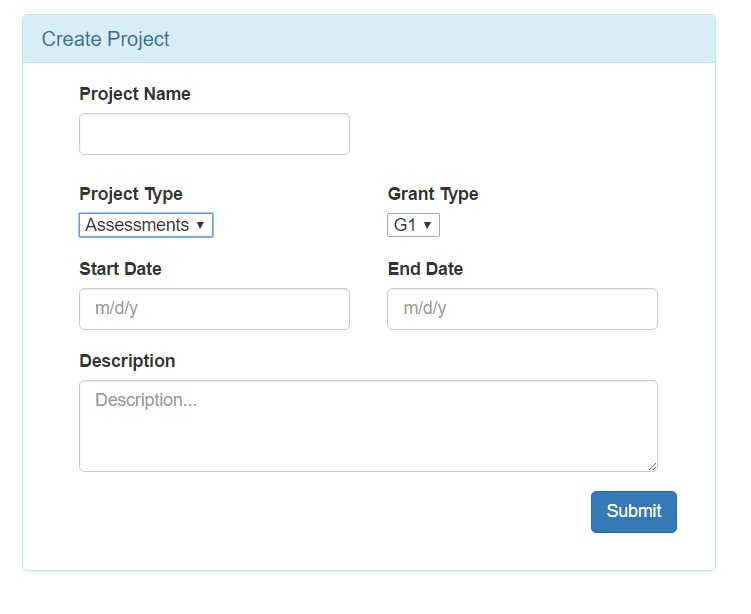
\includegraphics[scale=0.75]{dropdown} 


The image above shows the drop-down list which is populated from the database and displayed on the create project page.
\newline

\section{Team Evaluation}

\tab
Each member of our team contributes to the project in important ways. Kanna has taken the lead on communication and media. She has done an excellent job at staying on top of emails, meetings, and project media such as documents and presentations. Garrett has taken the more technical role of database management and PHP expert. Making sure the database is set up in a similar manner to the client’s will be crucial in the future. I have taken on the role of team captain. I like to make sure we are prepared and planning for future deadlines. I have worked on nearly all parts of the project and try to ensure that we keep the clients’ interests in mind.
\newline

\tab
Each member’s contribution has been equal but in different ways. We each contribute to the project whenever we can and make an effort to complete necessary tasks on time. We make sure to divide tasks evenly and complete them together. Although all three of us cannot always meet at the same time we always have at least two who can meet and work together. I think we have a strong team dynamic because of our participation. No one is absent from everything and our most productive moments are when we all come together. We have been able to keep positive relationships despite the large amount of stress that comes with a development project. Without all three group members, I believe this project would not have survived.
\newline

\section{Retrospective}

\begin{table}[H]
			\caption{Retrospective: Winter 2017}
			\begin{center}
				\begin{tabular}{| p{0.3\linewidth} | p{0.3\linewidth} | p{0.3\linewidth} | }
					\hline
					 \textbf{Positives} & \textbf{Deltas} & \textbf{Actions} \\ [0.5ex]
					%heading
					\hline
					Successful alpha release  & Implement form for loggin hours & Use template for assigning hours  \\
					\hline
					 Met with client and better understand their website  & Have Gantt display single project based on project type & Edit Gantt code to accomodate connecting it to a specific project type \\
					\hline
					 Completed beta release & Add more comments and double check consistency & Run project through lint until grade is A or higher \\
					\hline
					Strong team dynamic with good effort & Run usability tests and implement insights & Set up meeting with client to use our website and implement changes\\
					\hline
					 & Add overall polish to site  & Check for bugs by running tests and using the site\\
					\hline
					 & Entire site still dependant on our server and database & Create a plan for transferring files and tables to the EEC  \\
					\hline
				\end{tabular}
			\end{center}
			\end{table}

\section{10 Week Summary}

\begin{table}[H]
			\caption{Summarry: Winter 2017}
			\begin{center}
				\begin{tabular}{| p{0.3\linewidth} | p{0.3\linewidth} | p{0.3\linewidth} | }
					\hline
					 \textbf{Activities} & \textbf{Problems} & \textbf{Solutions} \\ [0.5ex]
					%heading
					\hline
					We will begin creating the website next week & We do not have access to the clients' database or web server & We will be using our own back end for now  \\
					\hline
					 We have our basic website layou implemented  & We do not have access to the clients' database or web server & We will be contacting the client again this week to try and get the information \\
					\hline
					 We have implemented the Gantt chart and a basic log in page & We do not have access to the clients' database or web server & We will meet with Tyler this coming week at the EEC\\
					\hline
					The client wants us to use our own database and server & log in page not functioning correctly & Troubleshoot log in page\\
					\hline
					Fixed log in and have tentative CSS theme & We are not ready for Alpha release & Schedule group coding sessions during next week\\
					\hline
					We have finished our Alpha release and completed midterm materials & Client needs an update & Schedule meeting with client to show them progress\\
					\hline
					 & Need to get our reports signed by client & Set up time to get client's signature\\
					\hline
					Outlined a plan to move our alpha release to beta & Some confusion about how the EEC uses the features we will be implementing for the beta release & Schedule meeting with client\\
					\hline
					Met with client and know how to implement beta level functionality & Need to finish beta release & Schedule coding sessions for next week\\
					\hline
					Finished our beta release and final progress report details & No problems & Plan for next term\\
					\hline
				\end{tabular}
			\end{center}
			\end{table}

\end{document}
